\documentclass[12pt,twoside]{article}

\usepackage[english]{babel}
\usepackage[utf8]{inputenc}
\usepackage{sansmathfonts}
\usepackage[T1]{fontenc}
\renewcommand*\familydefault{\sfdefault} %% Only if the base font of the document is to be sans serif
\usepackage{multicol,lipsum}
\usepackage{amsmath,cancel}
\usepackage{amssymb,amsthm,dsfont,mathrsfs}
\usepackage[colorinlistoftodos]{todonotes}
\usepackage{geometry}
\geometry{
a4paper,
total={170mm,257mm},
left=20mm,
top=15mm,
bottom=22mm,
}
\usepackage{natbib}
\usepackage{soul}
\usepackage{setspace}
\usepackage{hyperref}
\usepackage{xcolor}
\usepackage{graphicx}
\usepackage{tikz}
\usepackage{siunitx}
\graphicspath{ {imagens/} }
\usepackage{fancyhdr}
\pagestyle{fancy}
\renewcommand{\headrulewidth}{0pt}

\color{darkgray}
\newcommand{\T}[1]{\vspace{0.4cm}\textbf{\large#1}}
\newcommand{\TW}[1]{\textbf{\large#1}}

\newcommand{\TM}[1]{\vspace{0.2cm} \textbf{#1}}

\newcommand{\M}[1]{
\vspace{-0.6cm}
\begin{flalign*}
#1&
\end{flalign*}
\vspace{-0.6cm}
}


\definecolor{bluebell}{rgb}{0.25, 0.35, 0.89} 
\definecolor{laranja}{rgb}{0.87, 0.48, 0.25} 
\definecolor{verde}{rgb}{0, 0.54, 0.44} 
\definecolor{babypink}{rgb}{1, 0.42, 0.52} 
\definecolor{rosa}{rgb}{1, 0.72, 0.77} 
\definecolor{cinza}{rgb}{0.3, 0.3, 0.3}  
\definecolor{iris}{rgb}{0.25, 0.35, 0.89}  
\definecolor{babyblue}{rgb}{0.13, 0.59, 0.95}

\setlength\columnsep{30pt}

\setlength{\parindent}{0cm}
\setlength{\fboxrule}{1.3pt}  % <-- Aumenta a espessura

\newcommand{\Formula}[1]{
\begin{center}
\color{iris}
\fcolorbox{rosa}{white}{
\(
\begin{array}{c}
#1
\end{array}
\)
}
\color{cinza}
\end{center}
}

\begin{document}
\pagenumbering{gobble}


\includegraphics[width=4cm]{Logo2.png}
\begin{center}
    \textbf{\Huge \textcolor{bluebell}{Função Modular}}
\end{center}
\vspace{0.5cm}

\begin{multicols}{2}

% ── DEFINIÇÃO ────────────────────────────────────────────────────────────────
\TW{Definição}

O \textbf{módulo} (valor absoluto) de $x \in \mathbb{R}$ é:

\Formula{|x| = \begin{cases} x & x \geq 0 \\ -x & x < 0 \end{cases}}

$|5| = 5$, $\;|-3| = 3$, $\;|0| = 0$.

A \textbf{função modular} $f(x) = |g(x)|$ tem imagem em $[0,+\infty)$.

% ── GRÁFICO ───────────────────────────────────────────────────────────────────
\TW{Gráfico — Forma em V}

$f(x) = |x|$: vértice na origem; $f(x) = |x-h|+k$: vértice em $(h,k)$.

\begin{center}
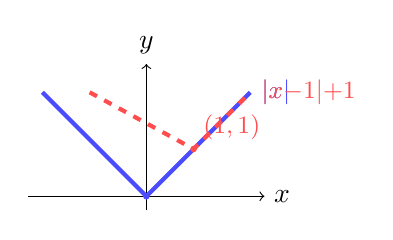
\begin{tikzpicture}[scale=0.6]
  \draw[->] (-2.5,0) -- (2.5,0) node[right] {$x$};
  \draw[->] (0,-0.3) -- (0,2.8) node[above] {$y$};
  % f(x) = |x|
  \draw[blue!70, line width=1.5pt] (-2.2,2.2) -- (0,0) -- (2.2,2.2)
        node[right, font=\small] {$|x|$};
  % g(x) = |x-1|+1, vertex (1,1)
  \draw[red!70, line width=1.5pt, dashed] (-1.2,2.2) -- (1,1) -- (2.2,2.2)
        node[right, font=\small] {$|x{-}1|{+}1$};
  \fill[blue!70] (0,0) circle (2pt);
  \fill[red!70]  (1,1) circle (2pt) node[above right, font=\small] {$(1,1)$};
\end{tikzpicture}
\end{center}

% ── EQUAÇÕES MODULARES ────────────────────────────────────────────────────────
\TW{Equações Modulares}

\Formula{|f(x)| = k \;\Rightarrow\; f(x) = k \;\text{ ou }\; f(x) = -k \quad (k \geq 0)}

$k < 0 \Rightarrow S = \emptyset$.

\TM{Exemplo 1 — $|2x-3| = 5$}

Caso 1: $2x-3 = 5 \Rightarrow x = 4$

Caso 2: $2x-3 = -5 \Rightarrow x = -1$

$$\boxed{S = \{-1,\; 4\}}$$

\TM{Dois módulos — $|f| = |g|$}

$$f(x) = g(x) \;\text{ ou }\; f(x) = -g(x)$$

% ── INEQUAÇÕES MODULARES ──────────────────────────────────────────────────────
\TW{Inequações Modulares}

\Formula{|f(x)| < k \;\Leftrightarrow\; -k < f(x) < k}

\Formula{|f(x)| > k \;\Leftrightarrow\; f(x) < -k \;\text{ ou }\; f(x) > k}

\TM{Exemplo 2 — $|x+1| \leq 4$}

$-4 \leq x+1 \leq 4 \Rightarrow -5 \leq x \leq 3$

$$\boxed{x \in [-5,\; 3]}$$

\TM{Exemplo 3 — $|3x-1| > 2$}

$3x-1 > 2 \Rightarrow x > 1$

$3x-1 < -2 \Rightarrow x < -\tfrac{1}{3}$

$$\boxed{x \in \left(-\infty,\; -\tfrac{1}{3}\right) \cup (1,\; +\infty)}$$

\fcolorbox{laranja}{white}{\parbox{0.85\linewidth}{
\small\textbf{Regra:} módulo \emph{menor} → intervalo (e); módulo \emph{maior} → união (ou).
}}

\end{multicols}

\lfoot{\scriptsize © Copyright, Pratique Já}
\cfoot{\large \textcolor{bluebell}{pratiqueja.com}}
\end{document}
